\chapter{Interfaces and Validation}
\section{Documentation Method}
This chapter describes implemented pages and API relationships from source inspection and selected application screenshots provided by the candidate on 17 November 2026. The captures illustrate visible interface states; they do not establish benchmark performance or successful completion of every available action. The navigation diagram summarizes the source-derived route structure.
\begin{figure}[htbp]\centering\begin{tikzpicture}[node distance=0.7cm]
\node[box,text width=9cm] (l) {Login / registration};
\node[box,below=of l,text width=9cm] (s) {Protected shell: navbar, sidebar, theme, console};
\node[box,below left=1cm and -1cm of s,text width=4cm] (a) {Administrative navigation\\Dashboard, directory, audit};
\node[box,below right=1cm and -1cm of s,text width=4cm] (u) {Authenticated navigation\\Anomalies, risk, logs, AI};
\draw[flow](l)--(s);\draw[flow](s)--(a);\draw[flow](s)--(u);
\end{tikzpicture}\caption{Source-derived navigation; backend authorization still applies.}\end{figure}

\section{Authentication and Navigation}
Login is outside the protected layout. Authentication context saves token and safe user data in browser local storage. The shared client sends bearer credentials and clears authentication state after relevant unauthorized responses. Registration creates an ordinary user.

Persistence survives a page refresh, but local storage can be accessed by scripts running within the page. Tests should cover token expiry, injected scripts, and malformed stored data. Frontend route guards assist navigation but cannot replace API authorization.

\section{Dashboard and Anomalies}
The dashboard route is administrator-only. Its combined metrics provide entry points to accounts or incidents requiring investigation. The anomalies API supports filtering, pagination, identifier lookup, and user-scoped views. Investigation should begin with stored rule type, description, and linked event metadata before considering generated explanations.

An anomaly alone does not prove an account was compromised. For example, a changed IP can reflect legitimate movement or network changes. The interface should support comparing related events and account context rather than implying that every rule match is an attack.

\section{Risk and Login Logs}
The risk view uses the score and its 24-hour horizon. A high score indicates accumulated rule weights; a low score may also reflect absent or expired telemetry. The logs page lists events and includes an administrative simulation form. The form creates a supplied telemetry record and invokes rules; it does not perform a real password attempt or network attack.

Synthetic records should be identified in demonstrations so they are not mistaken for genuine authentication evidence. Testing should compare the explicit ingestion path and real authentication recording because their timestamp and input sources differ.

\section{Directory, Audit, and Console}
The users page supports administrator account operations and active-state management. The audit page displays selected persisted security events. The Winston console component supplies browser diagnostics and API activity. Console output and database audit events have different purposes and should not be described as a complete forensic trail without coverage and integrity tests.

\section{AI Workspace}
The AI page selects investigator, containment operator, or collaborative behavior. It accepts prompt, context, queued steering, and follow-ups, then copies queue values into the request before submission. Returned steps show tool invocations and outcomes alongside final Markdown text and availability indicators.

Fallback output can still rely on real application tools. Absence of live inference does not automatically make every registry action a dry run. Validation must establish what the fallback planner selects and what permissions are enforced.

\clearpage\section{Application Screenshots}
Six captures were selected to show the entry point, overall monitoring, event investigation, personal account scope, and AI workspace. They are reproduced from candidate-provided screenshots without changing the displayed content. Counts and scores describe the captured demonstration state, not evaluation results.

\begin{figure}[!ht]\centering
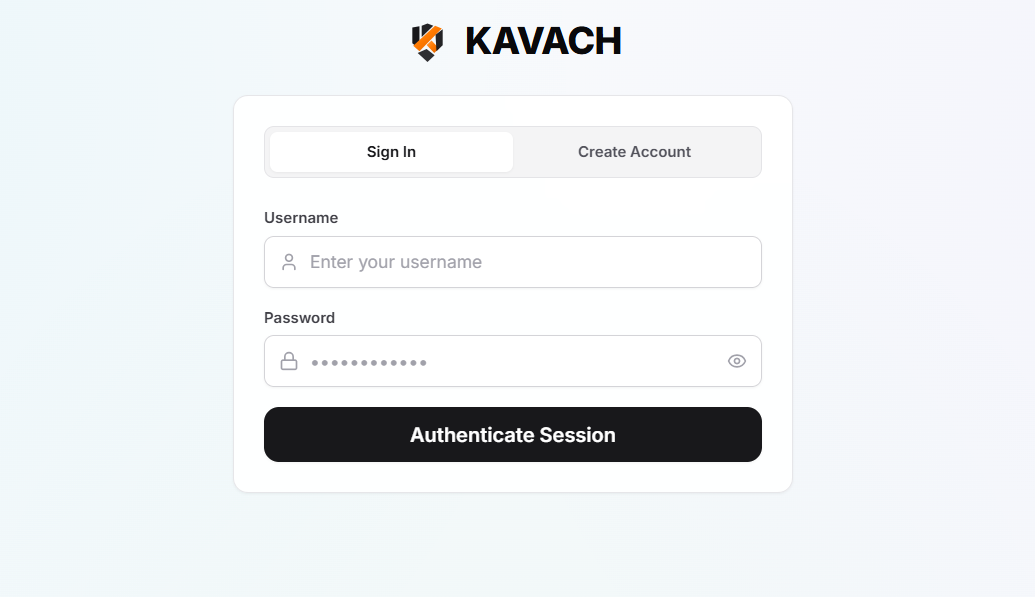
\includegraphics[width=.75\textwidth]{images/screenshot-login.png}
\caption{Sign-in interface with account-registration tab and authentication form.}\label{fig:screen-login}
\end{figure}

\begin{figure}[!ht]\centering
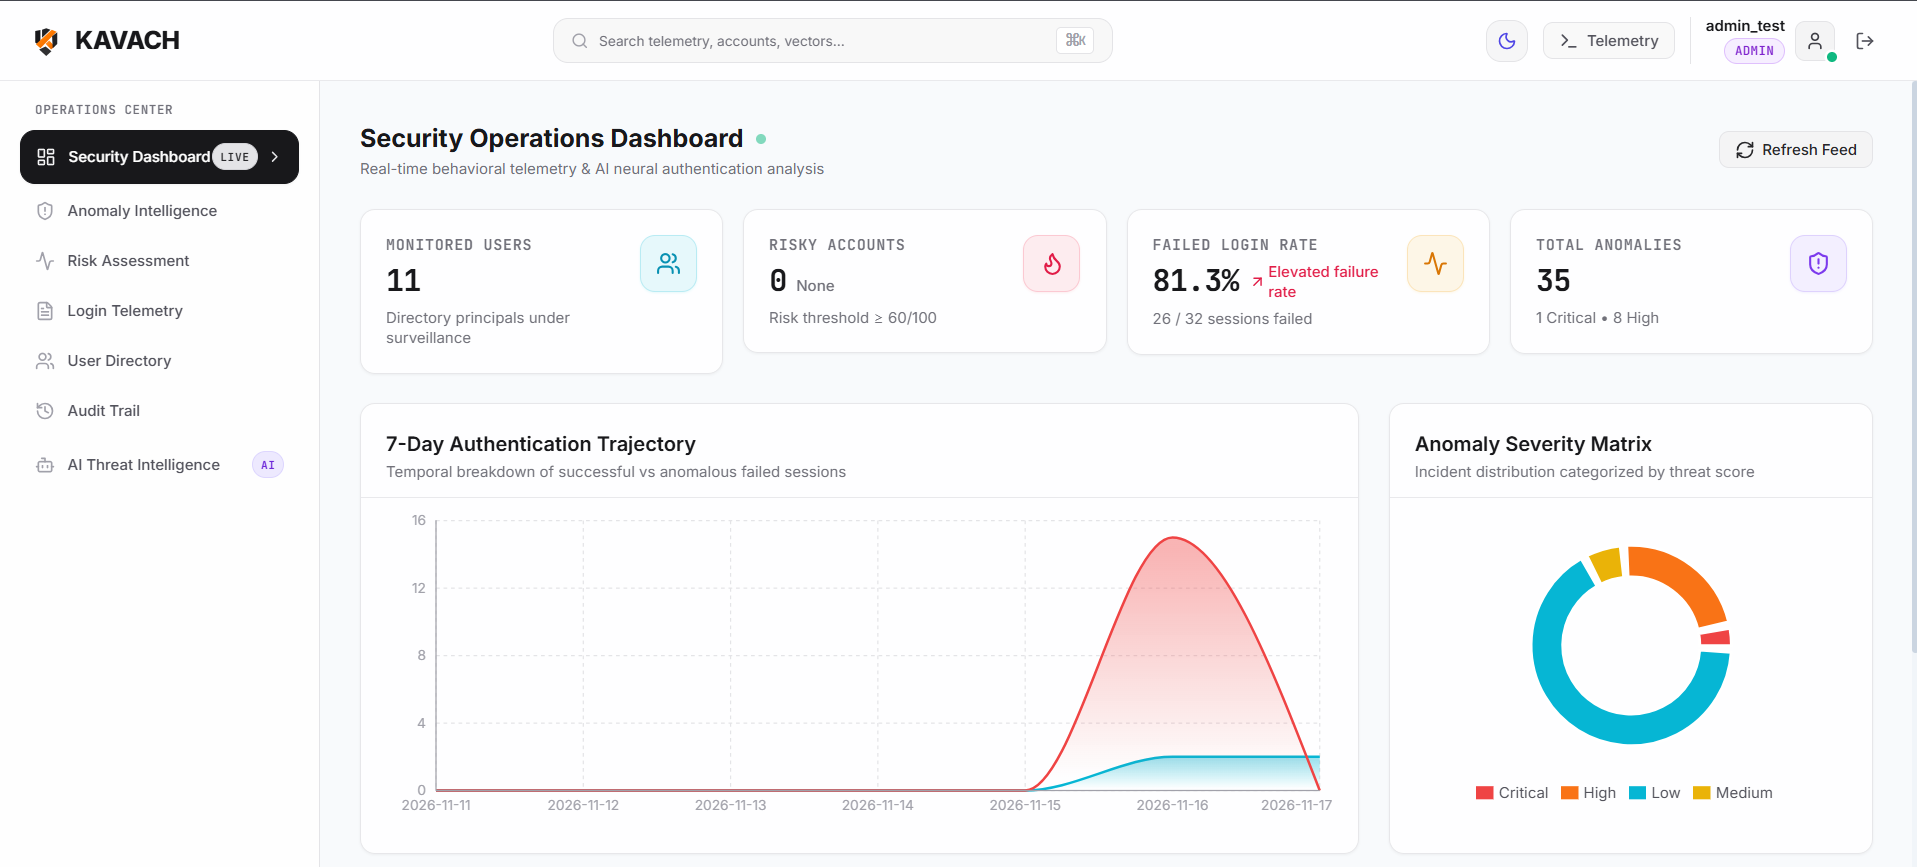
\includegraphics[width=\textwidth]{images/screenshot-dashboard.png}
\caption{Administrator dashboard: account counts, login outcomes, trend, and anomaly severity.}\label{fig:screen-dashboard}
\end{figure}

\clearpage\subsection{Anomaly Investigation and Login Telemetry}
The anomaly view exposes rule matches and per-alert weights, while the telemetry view shows the underlying login-event fields. Filters and action buttons are visible entry points; the captures do not show the outcomes of clicking those actions.

\begin{figure}[!ht]\centering
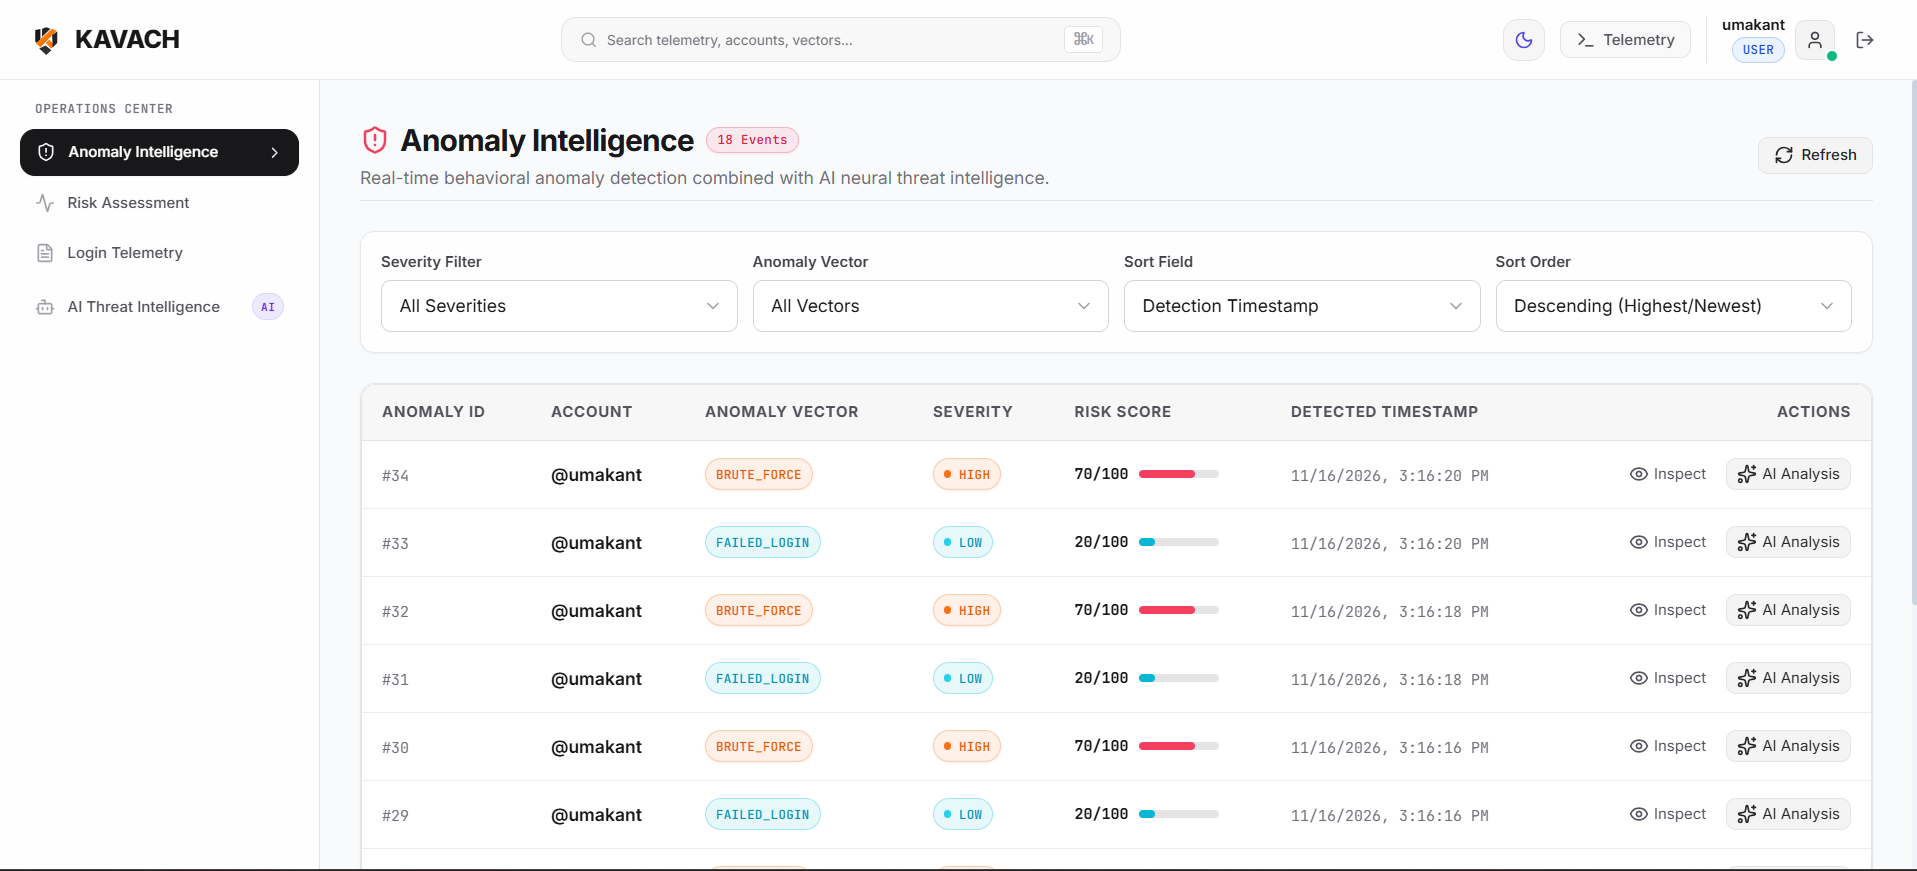
\includegraphics[width=\textwidth]{images/screenshot-anomalies.png}
\caption{User-scoped anomaly list with filters, rule types, severity, and alert weights.}\label{fig:screen-anomalies}
\end{figure}

\begin{figure}[!ht]\centering
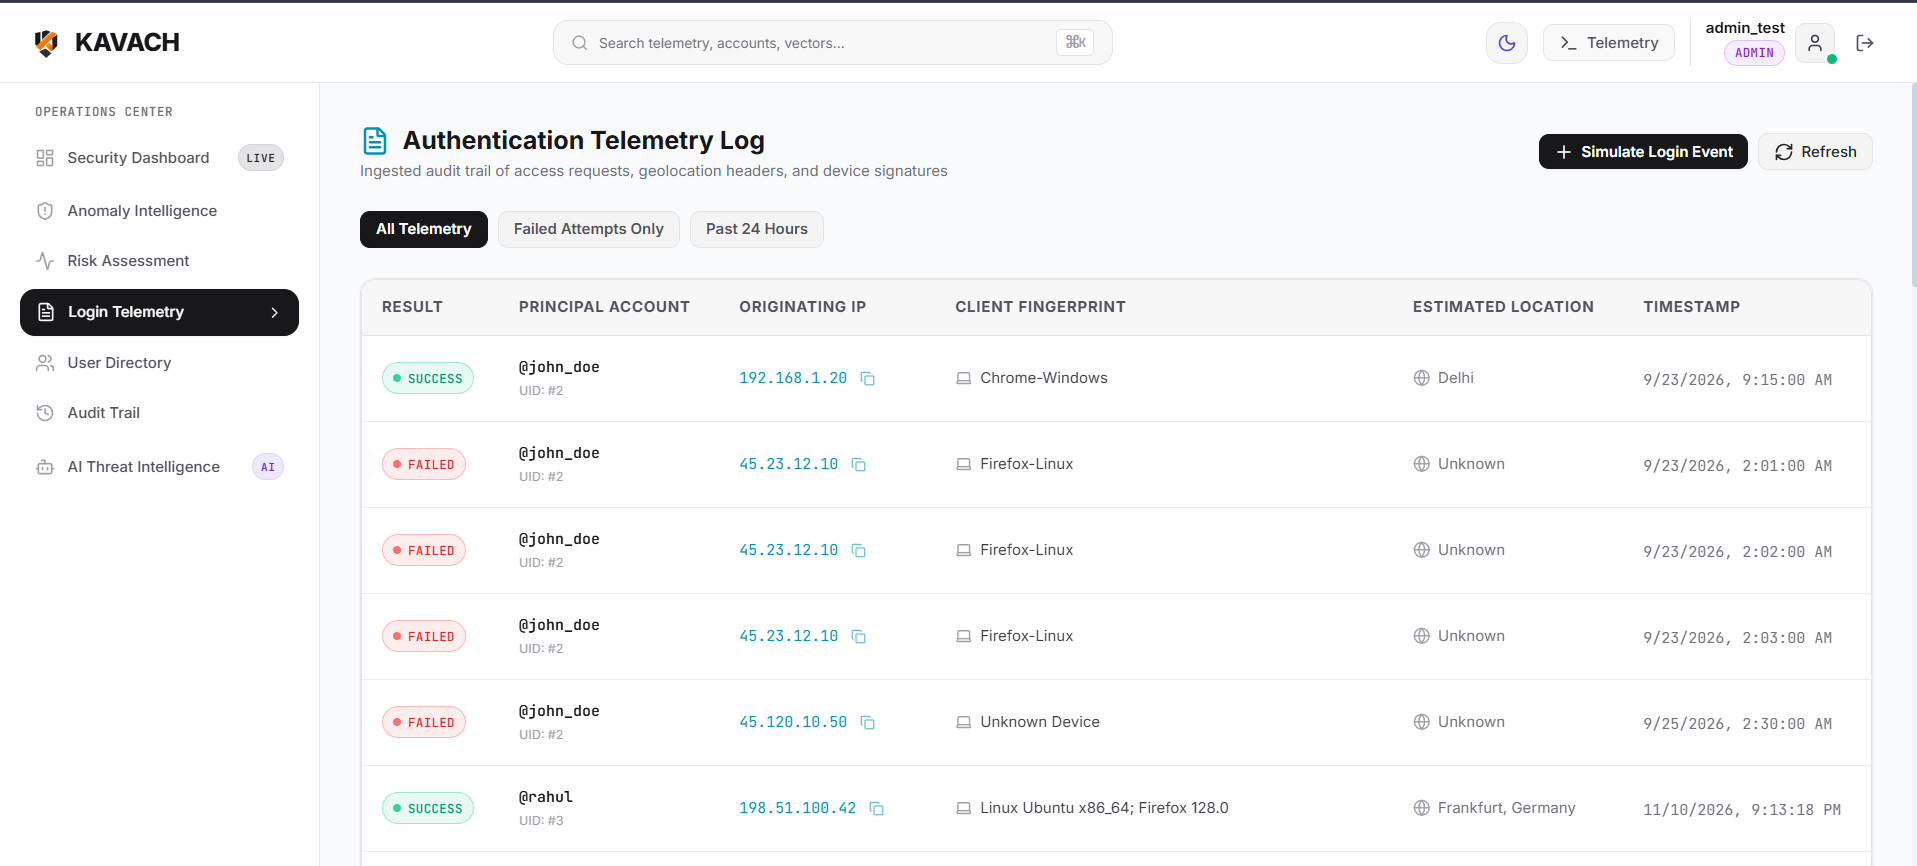
\includegraphics[width=\textwidth]{images/screenshot-telemetry.png}
\caption{Login telemetry showing successful and failed events with account and client metadata.}\label{fig:screen-telemetry}
\end{figure}

\clearpage\subsection{Personal Risk and AI Workspace}
The personal view displays the signed-in account's risk profile. Historical anomaly counts and the recent 24-hour risk score use different horizons. Interface subtitles such as ``Bayesian'' or ``neural'' do not alter the fixed-rule detector and additive score documented in Chapter 4. The AI capture shows its initial console state rather than a completed model or tool execution.

\begin{figure}[!ht]\centering
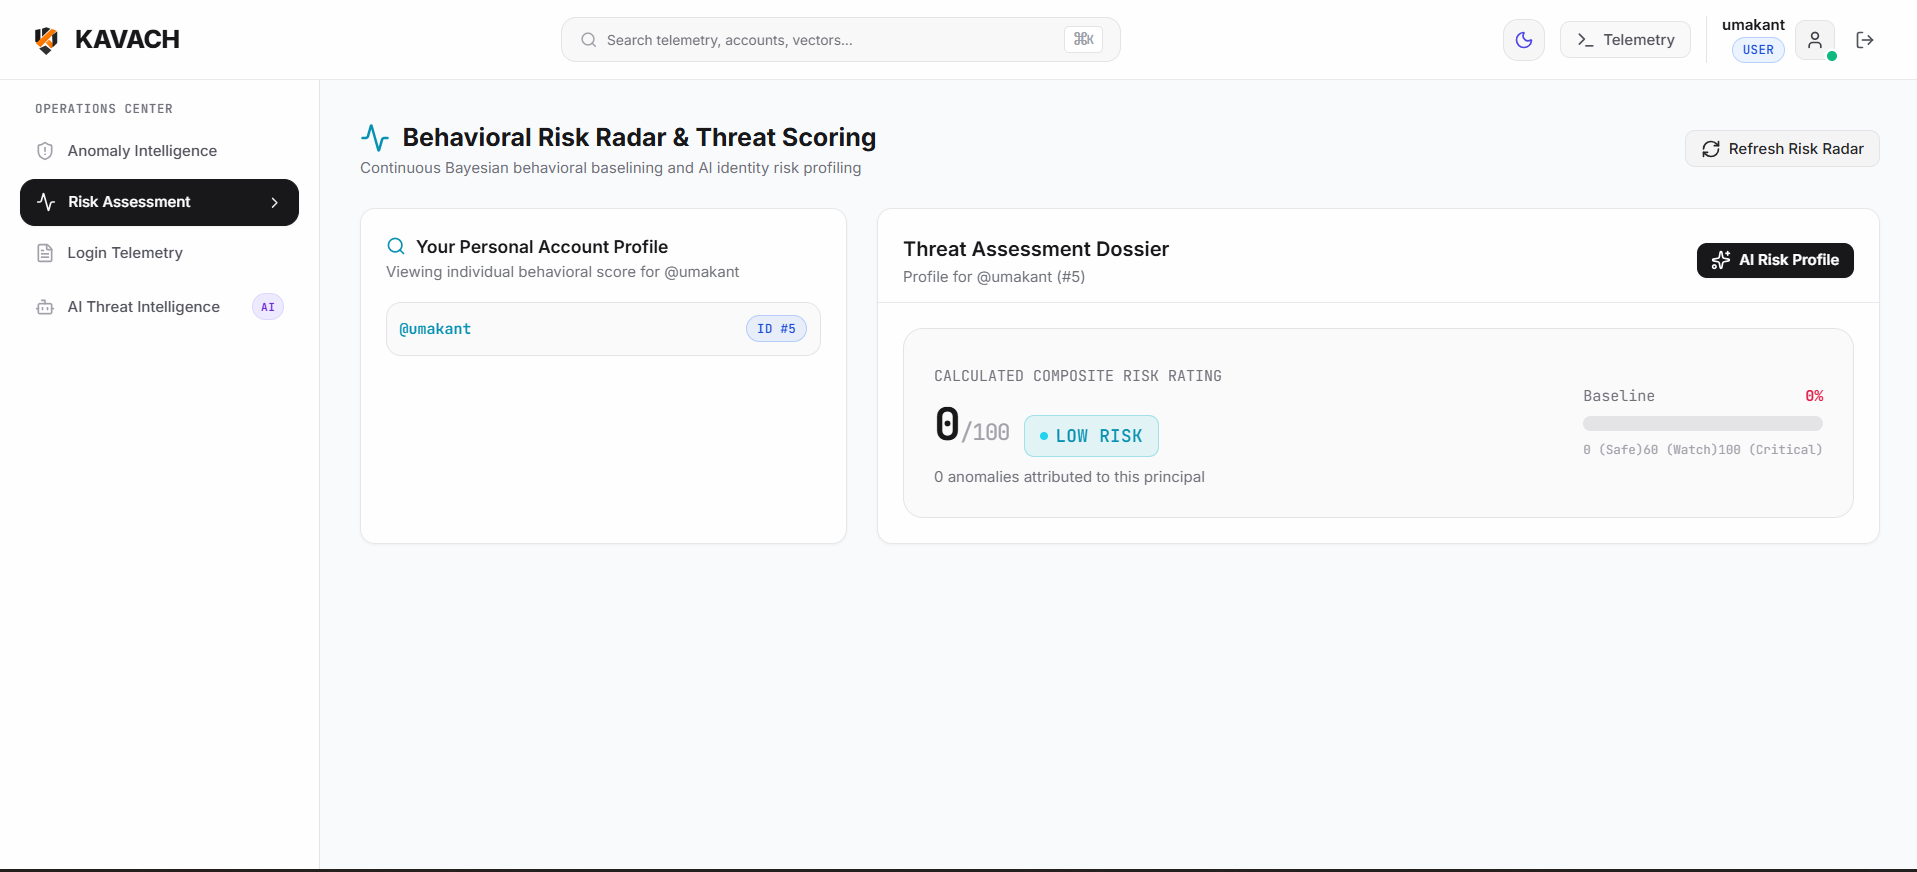
\includegraphics[width=\textwidth]{images/screenshot-personal-risk.png}
\caption{Personal risk view for the USER account, showing the displayed score and profile.}\label{fig:screen-risk}
\end{figure}

\begin{figure}[!ht]\centering
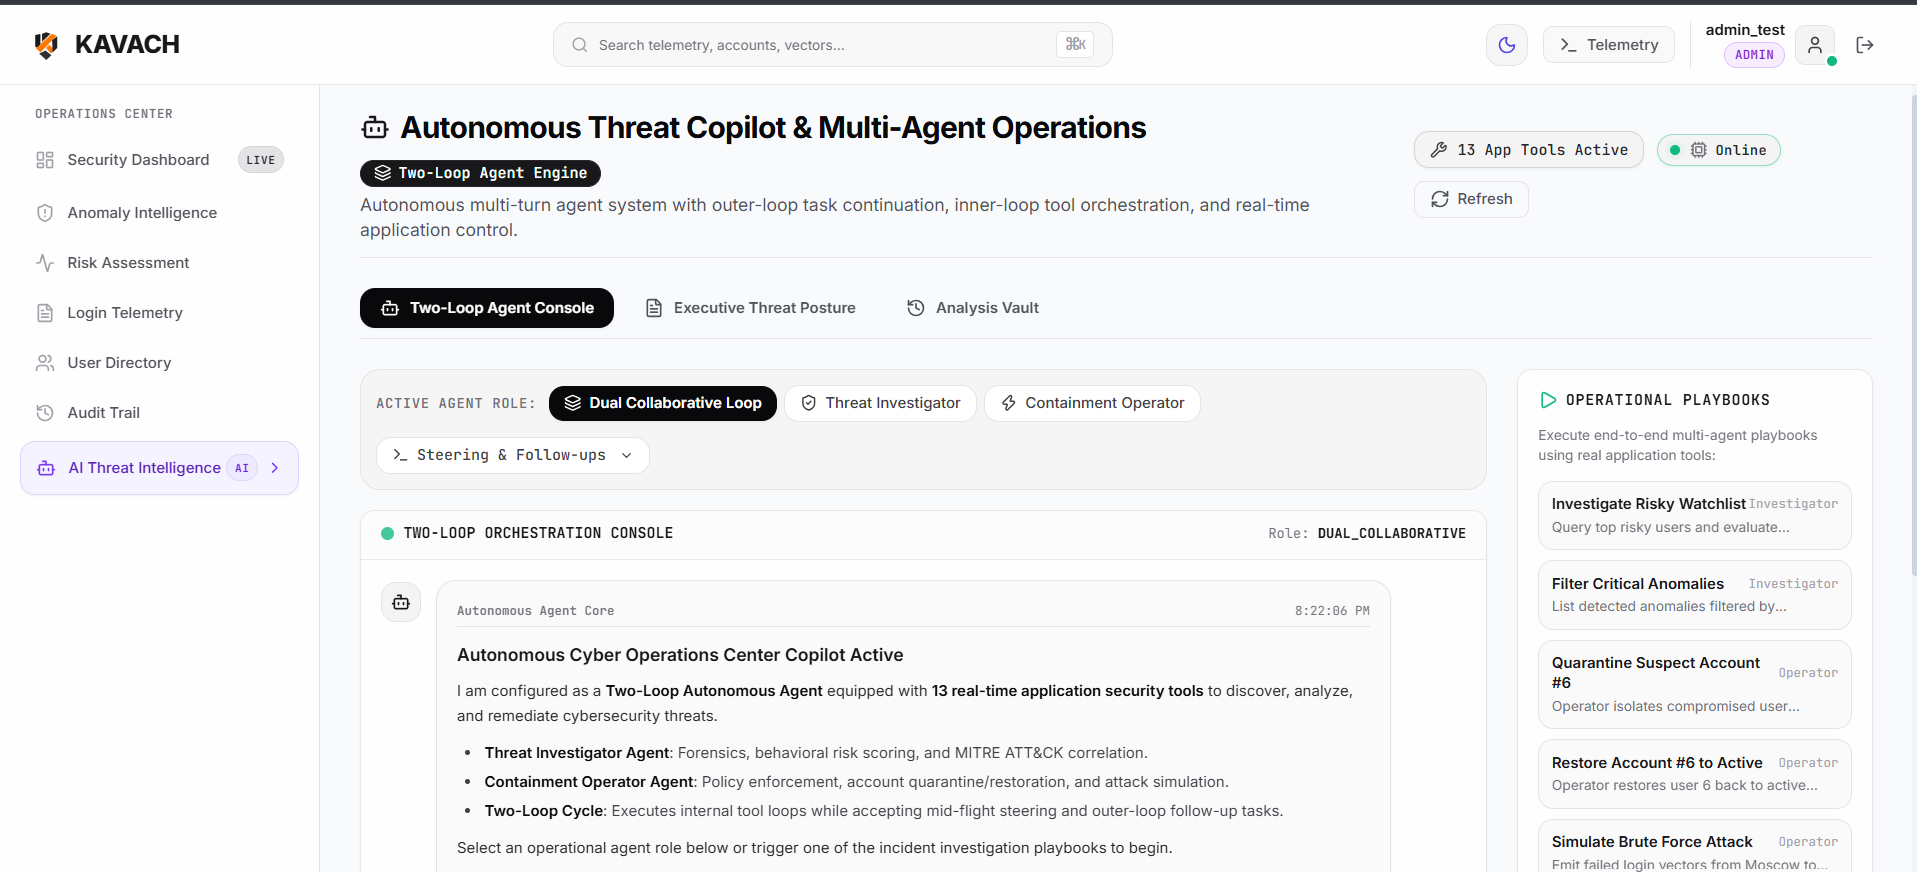
\includegraphics[width=\textwidth]{images/screenshot-ai-console.png}
\caption{AI workspace with agent-role selection, a 13-tool indicator, and operational playbooks.}\label{fig:screen-ai}
\end{figure}


\clearpage\section{Validation Status}
The repository contains one Spring Boot context-loading test. No rule-specific test-run results, labelled dataset, or load-test output was supplied. Source inspection and the candidate's screenshots support the implementation and interface descriptions. The screenshots are visual examples rather than a controlled execution of the validation plan. Table~\ref{tab:tests} lists proposed tests with expected behavior derived from the implementation; these are not recorded pass results.
\begingroup\small\setstretch{1.1}\setlength{\parskip}{0pt}
\begin{longtable}{>{\raggedright\arraybackslash}p{0.9cm}>{\raggedright\arraybackslash}p{6.1cm}>{\raggedright\arraybackslash}p{7cm}}
\caption{Functional validation plan; execution pending.}\label{tab:tests}\\\toprule ID & Input / action & Expected behavior to verify\\\midrule\endfirsthead
\toprule ID & Input / action & Expected behavior to verify\\\midrule\endhead
T1 & Register unique credentials. & Active USER, encoded password, safe response, audit event.\\
T2 & Repeat username or email. & Conflict and no duplicate account.\\
T3 & Valid password for active user. & JWT, success telemetry, applicable contextual rules.\\
T4 & Incorrect password for known user. & Unauthorized; failed telemetry and failed-login anomaly.\\
T5 & Unknown username. & Audit failure; no user-linked login record.\\
T6 & Inactive account attempts login. & Forbidden; failed telemetry and inactive-user anomaly.\\
T7 & Events at 04:59 and 05:00. & Unusual-time alert only before 05:00.\\
T8 & First event, repeated values, unseen IP/device. & No initial new-value alerts; later unseen values trigger.\\
T9 & Four then five failures in window. & Fifth qualifying failure adds brute-force anomaly.\\
T10 & Reanalyse identical login event. & No duplicate event/user/rule anomaly in sequential execution.\\
T11 & Weight totals 29, 30, 59, 60, 79, 80, 120. & Correct boundary tiers; score capped at 100.\\
T12 & Move anomaly detection time beyond 24 hours. & Expired anomaly excluded from risk.\\
T13 & Deactivate account with issued JWT. & Subsequent protected request rejected.\\
T14 & Make live inference unavailable. & Deterministic fallback with accurate status and outcomes.\\
T15 & Submit steering and two follow-ups. & Inner context consumes steering; outer cycles consume follow-ups.\\\bottomrule
\end{longtable}
\endgroup

\section{Security and Boundary Tests}
Test a USER requesting another account's logs, anomalies, and risk. Test directory changes through both direct REST and agent tools. Unauthorized data or actions should be denied. Tool-path tests matter because the inspected source uses differing call boundaries.

Exercise missing arguments, negative limits, oversized strings, invalid statuses, nonexistent IDs, and unknown tools. Feed malformed model JSON, provider errors, and misleading instructions inside tool results. Check failure during multi-step writes and concurrent anomaly insertion.

Time tests should include the exact ten-minute boundary, a backdated event with later failures already stored, and a recently inserted historical event. These distinguish strict ``after'' predicates, absent upper bounds, and login time from detection time.

\section{Empirical Evaluation Plan}
After functional validation, use a labelled corpus combining representative ordinary activity and controlled suspicious cases. Calculate precision and recall per rule and for the combined alert stream. Measure persistence, detection, dashboard queries, and model requests separately. Record hardware, database size, versions, concurrency, provider mode, and repeated runs.

Keep deterministic-fallback results separate from live-model results. Until measurements exist, the supported conclusion is that the source implements an inspectable monitoring workflow, with empirical effectiveness still to be established.
